La expansi\'on en ondas planas puede contener un n\'umero infinito de t\'erminos haciendo dif\'icil su manejo computacional. Para reducir el n\'umero de ondas planas se define una energ\'ia de corte $E_{cut}$

\begin{equation}
    E_{cut} \ge \frac{1}{2} |K + G|^{2}  \textup{ ,}
\end{equation}

\noindent todas las ondas planas por debajo de este limite son tomadas en cuenta en la expansi\'on. Una forma esquematica de ver esta energ\'ia de corte se observa en la figura \ref{EnergiaCorte}.


\begin{figure}[H]
    \centering
    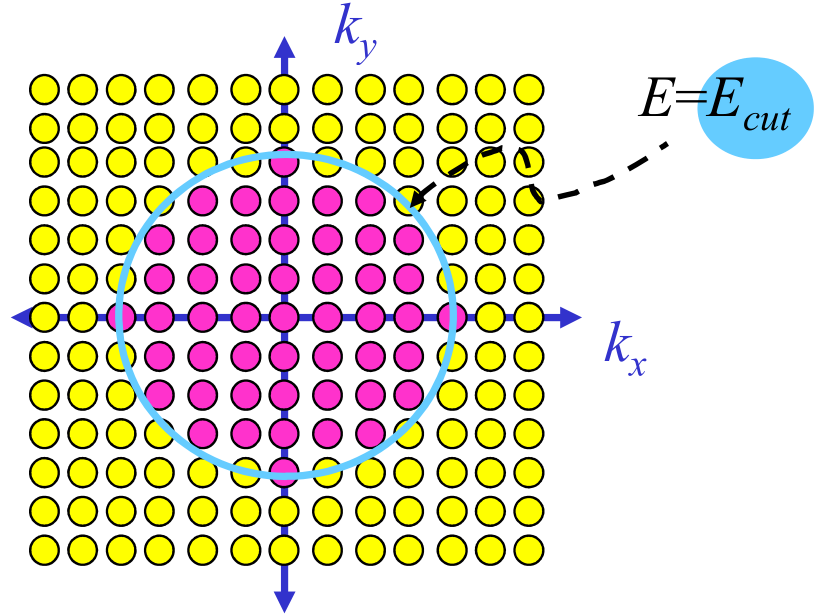
\includegraphics[width=0.6\linewidth]{contenido/calculos_computacionales/energia_corte/img_corte/EnergiaCorte}
    \caption{Representaci\'on esquem\'atica de la energ\'ia de corte.}
    \label{EnergiaCorte}
\end{figure}

\noindent La energ\'ia de corte es un par\'ametro que debe ser calculado espec\'ificamente para cada sistema tratado.